\documentclass[letter,oneside]{memoir}
\usepackage{bstyle}
\begin{document}
\chapter{Complex Numbers}
\section{Introduction}
Mathematicians did not begin by defining numbers: they worked with them. The consciousness of the number system grew, and at the beginning of the seventeenth century - the most important century up to that time in the history of human thought - algebra, as we know it in the requirements for admission to college, was completed. True, it was very far from complete when we look at the definition of number. But the formal processes were recognized, and science could go on. It is hard to imagine what the Greek mind might not have accomplished if Euclid and Archimedes could have passed the entrance examinations for Pei ta in Algebra\footnote{For an interesting account of the beginnings of arithmetic and algebra cf. David Eugene Smith: \begin{em}The Teaching and History of Elementary Mathematics\end{em}. A systematic development of the number system, so far as real numbers are concerned, is found in Osgood: \begin{em}Functions of Real Variables, Chap. II\end{em}.}.

Nor did mathematicians worry much over the foundations in algebra. The formal processes were enough for the next step: 
\begin{align*}
	A+B&= B+A\\
	A+(B+C)&=(A+B)+C\\
	AB &= BA\\
	A(BC) &= (AB)C\\
	A(B+C) &= AB + AC
\end{align*} But then came the question of solving equations. The equation 
\[
ax=b, \quad a\neq 0
,\] could always be solved. The quadratic 
\[
ax^2+bc+c=0
\] admitted the formal solution 
\[
x=\frac{-b\pm \sqrt{b^2-4ac} }{2a} 
.\]

But what if $b^2-4ac$ is negative? The algebrists of the sixteenth and seventeenth century took the hurdle. 
\begin{align*}
	x^2+1&=0\\
	x&=\pm \sqrt{-1} 
\end{align*} They did not define $\sqrt{-1} $; they treated it like any other letter of algebra, replacing its square, however, by $-1$: 
\begin{align}
	a+b\sqrt{-1} +c +d \sqrt{-1} &= (a+c)+(b+d)\sqrt{-1} \\
	(a+b\sqrt{-1} )(c+d\sqrt{-1}) &= ac+ad\sqrt{-1} +bc\sqrt{-1} +bd\left(\sqrt{-1}  \right) ^2=ac-bd+(ad+bc)\sqrt{-1}\label{1.2mult} 
\end{align} 

The results were of far reaching importance. Algebraic geometry came into being. An ellipse may and may not be cut by a line its plane. It is not an exception for a line to fail to meet the curve. As many lines fail to meet it as meet it, so to speak. But when imaginaries are introduced, and the plane is suitably extended, \emph{every} right line cuts the ellipse, and there are in general two points of intersection. 

In algebra, the Fundamental Theorem emerged, namely, the fact that every algebraic equation has a root. 

The modern developments of Arithmetic are more concerned with numbers which are not real, than with those which are. 

But it was in Analysis that the most spectacular resets were achieved. The mathematicians of Euler's time had observed that when $\sqrt{-1} $ is introduced, the trigonometric functions on the one hand, and the logarithm and the exponential on the other, unite to form one family:
\begin{align}
	\sin \phi &=\frac{e^{\phi i}-e^{-\phi i}}{2i} \\
	\cos \phi &= \frac{e^{\phi i}+e^{-\phi i}}{2} 
\end{align} 

where we write with Euler:
\[
i=\sqrt{-1} 
.\] And again:
\[
\tan ^{-1}x=\frac{i}{2}\log \frac{i+x}{i-x} 
.\] If we set 
\[
z=x+iy 
\] we find:
\[
	e^{x}=e^x\pbr*{\cos y +i\sin y } 
.\] The student will do well at this point to turn to the Author's Advanced Calculus and study again Chap. XX.

One further illustration of the formal use of imaginaries before leaving this part of the subject. The linear differential equation with constant coefficients:
\begin{equation}\label{1.1difeq}
\frac{d^2y }{dx^2} +2a \frac{dy}{dx} +by =0
\end{equation} 
can be solved by setting 
\[
y=e^{mx}
\] and then determining $m$ from the equation:
\begin{equation}\label{1.1sol}
m^2+2am+b=0
\end{equation} If $m_1$ and $m_2$ are roots of this equation, then 
\[
y =c_1e^{m_1x}+c_2e^{m_2x}
\] is the general solution of \ref{1.1difeq}. But what if the roots of \ref{1.1sol} are imaginary? 

Setting 
\begin{equation}\label{1.1c}
c=\sqrt{b-a^2} 
\end{equation} we find two new solutions:
\[
y=e^{-ax+cix}, \qquad y_2=e^{-ax-cix}
,\] both of these are imaginary, and so useless for any practical purposes. 

Now, the sum of any two solutions of \ref{1.1difeq} is also a solution. If, then, we write:
\begin{align*}
	y_1&=e^{-ax}\cos cx+ie^{-ax}\sin cx\\
	y_2&=e^{-ax}\cos cx-ie^{-ax}\sin cx
\end{align*} we find:
\[
Y_1=y_1+y_2=2e^{-ax}\cos cx
.\] And similarly 
\[
Y_2=y_1-y_2=2ie^{-ax}\sin cx
.\] Moreover, the product of \ref{1.1difeq} by a constant is also a solution, and so we are led to the two solutions:
\begin{equation}
u_1=e^{-ax}\cos cx, \qquad u_2=e^{-ax}\sin cx
\end{equation} 
All this is seventeenth and eighteenth century mathematics, and can make no claim to rigor. There is no foundation for it to rest on. It is crass formalism. Nevertheless, this formal work has produced a concrete result. Here are two real functions which have emerged. Now the test of whether a given function is a solution of a differential equation is not the process whereby the function was obtained - we may have found it in the street. The test is: Does it satisfy the differential equation? Let us see.
\begin{align*}
	u_1&=e^{-ax}\cos cx\\
	\frac{du_1}{dx} &=-ae^{-ax}\cos cx-ce^{-ax}\sin cx\\
	\frac{d^2u_1}{dx^2} &=\pbr*{a^2-c^2} e^{-ax}\cos cx+2ace^{-ax}\sin cx
\end{align*} On multiplying the first of these equations by $b$, the second by $2a$ and adding, remembering \ref{1.1c}, the right-hand side reduces identically to $0$. Hence $u_1$ is a solution, in spite of the shady methods by which it was obtained. And similarly for $u_2$. 

This example illustrates one side of the eighteenth century use of imaginaries. A large number of definite integrals, like 
\[
\int \limits_{0}^{\infty} \frac{\sin x}{x}  \: dx 
\] were evaluated in this manner. In fact, the attempt to put his latter class of formal developments on a firm basis led Cauchy, in one of his earliest papers, in 1814, to lay the foundations of the Theory of Functions.

Two other topics of eighteenth century mathematics should be mentioned before we leave this brief sketch of the main ideas which led up to the modern Theory of Functions of a Complex Variable. First, the problem of \emph{cartography}, or map making. This is the question of transforming one curved surface on another in such a manner that small figures on the one surface will go over in approximately similar figures of the other surface. A necessary condition is, that angles be preserved; i.e, the angles between two intersecting curves on the one surface and the angle between their images on the other surface, must be equal. Conversely, this condition is sufficient. Such a transformation is called \emph{isogonal}, and the map is called \emph{conformal}. There are two principal maps of the earth, which are used in geography, namely, Mercator's Chart and Stenographic Projection; cf. Chaps. II, \S 10 and III, \S 6. 

In particular, the surfaces may be planes. If a system of Cartesian coordinates $(x,y)$ be chosen in the one plane, and a suitable Cartesian system  $(u,v)$ in the other, then the condition for a conformal mapping is that the following differential equations be true:
\begin{equation}\label{conformal}
\frac{\partial u}{\partial x} =\frac{\partial u}{\partial y} , \qquad \frac{\partial u}{\partial y} =-\frac{\partial v}{\partial x} 
\end{equation} 
These are known as the \emph{Cauchy-Riemann Differential Equations}. They have come to us as the definition of conformal mapping. They appeared, however, still earlier, in a paper of Clairaut of the year 1743, on the Figure of the Earth, in his study of a two-dimensional flow of an incompressible fluid; cf. Chap II, \S 4. 

Thus even more fundamental than Geometry in the development of Analysis has been the science of Mechanics and Mathematical Physics. Nor was it in the study of hydromechanics alone. The first half of the nineteenth century brought a tremendously stimulating contribution to mathematical physics in the investigation of Fourier on the flow of heat in conducting substances. The flow of electricity in conductors obeys parallel laws, and the two problems are mathematically identical. Thus the work of Fourier helped to pave the way for Maxwell in his study of electricity and magnetism, in the second half of the last century. 

When the flow is two-dimensional and is steady, the temperature $u$ satisfies \emph{Laplace's Equation}:
\begin{equation}\label{laplace}
\frac{\partial^2 u}{\partial x^2} +\frac{\partial^2 u}{\partial y^2} =0
\end{equation}
So important did Maxwell consider this case that he published accurately drawn figures illustrating particular cases of flow, in his great work on Electricity and Magnetism. These and similar examples have proved useful to electrical engineers, and hold a permanent in this applied science. 

By an \emph{analytic function of a complex variable}:
\[
	w=f(z)
,\]where 
\[
z=x+yi, \qquad w=u+vi
\] is meant a function which has a derivative; i.e, 
\[
	\lim\limits_{\Delta z \to 0} \frac{f(z_0+\Delta z)-f(z_0)}{\Delta z} 
\] shall exist, no matter how $\Delta z$ approaches $0$. A necessary condition for this limit to exist is, that $u$ and $v$ satisfy the Cauchy-Riemann Differential Equations \ref{conformal}, the partial derivatives being continuous functions. 

This condition is conversely sufficient: If $u$ and $v$ are two real functions which have continuous first partial derivatives in a two-dimensional region $S$ of the $(x,y)$ plane, and if the Cauchy-Riemann Differential Equations are satisfied in $S$, then the complex function
\[
	w=u+vi=f(z)
\] will have a derivative at each point of $S$. Moreover, the functions $u$ and $v$ will then possess derivatives of all orders, and $u$ will satisfy Laplace's Equation \ref{laplace}, as is seen at once by eliminating $v$. 

Thus the real part of an analytic function of a complex variable satisfies Laplace's Equation. Conversely, every every solution $u$ of Laplace's Equation leads to a complex conjugate function $v$ and the two together satisfy the Cauchy-Riemann Differential Equations. So the Theory of Functions of a Complex Variables is in principle coextensive with the theory of Laplace's Equation. 

It is of historical interest to trace the origins of the Theory of Functions of a Complex Variable to the great branches of Mathematical Physics and of Geometry. It is no less important for a sure sense of scientific values, to recognize how deep these roots go down. Not the theory of unctions alone, but the mathematical physics of the future will take its origin in these same sources. We are studying something universal when we make these theories a part of our mental equipment and our habits of thought. 

\section{The System of Complex Numbers}

The system of real numbers having been developed according to the method of Dedekind or Cantor, or in some other way, a new class of objects is defined by the mark $(a,b)$ where $a$ and $b$ are any two real numbers. 

\emph{Equality}: Two of these numbers,
\[
	A=(a,b), \quad B=(c,d)
\] shall be said to be equal if
\[
a=c, \, b=d
.\] We write:
\[
A=B
.\] If $A=B$, then $B=A$. Moreover, if $A=B$ and $B=C$, then $A=C$.

The relation of $<$ and $>$ are not defined. But the fact that $A$ and $B$ are not equal may be expressed in the form:
\[
A\neq B
.\] By a \emph{combination} of two of these numbers is meant a rule, whereby a third number is determined. These combinations lead eventually to \emph{addition} and \emph{multiplication}; but we will not speak of them as such for the present, since these words have connotations which would confuse the main ideas. We will think of a combination rather as a function of two independent variables:
\[
	C=f(A,B)
;\] a very simple function, which we proceed to define. 

\emph{Addition}: Let
\[
	A=(a,b), \quad B=(c,d)
\] be any two numbers of the system. By the \emph{first combination} is meant the mark:
\[
A\oplus B
.\] To it is attached the value:
\[
C=A\oplus B
\] where
\[
	C=\pbr*{a+c, b+d} 
.\] Thus
\begin{equation}\label{oplus}
	(a,b)\oplus (c,d)= (a+c, b+d).
\end{equation}

The first combination obeys the Commutative Law:
\[
A\oplus B = B\oplus A
.\] It also obeys the Associative Law:
\[
	A\oplus \pbr*{B\oplus C} =\pbr*{A\oplus B} \oplus C
.\] \emph{Subtraction:} The first combination admits an inverse defined as follows. Let $A=(a,b)$ and $B=(c,d)$ be any two numbers of the system, and let it be required to determine a number $X=(x,y)$ such that
\[
A\oplus X=B
.\] the solution is given by the equations:
\[
a+x=c, \quad b+y=d
.\] Thus one and only one number $X$ exist, satisfying the condition. We write:
\[
X=B\ominus A
.\] The number
 \[
	 A_0=(0,0)
\] has the property that
\[
A\oplus A_0=A_0\oplus A = A
,\] no matter what number $A$ may be. Moreover, it is unique.

\emph{Vectors}: The number $A=(a,b)$ admits \emph{two} important geometrical interpretations:
\begin{enumerate}[i.]
	\item It can be represented by the point of the plane of coordinate geometry, whose coordinates are $(a,b)$.
	\item It can be represented by the \emph{vector} whose initial point is the origin of coordinates, and whose terminal point is $(a,b)$ : or by any other equal vector.
\end{enumerate}
The representation of complex numbers by the points of a plane, or by vectors in a plane, came into mathematics through the memoire of Argand, Paris, 1806. The method was known to Gauss and is contained implicitly in his doctoral thesis of 1799. The earliest publication is that of Gaspar Wessel, 1797/99. cf, \emph{Funktionentheorie} I, p.225.


\begin{figure}[htbp]
	\centering
	\scalebox{1.5}{%
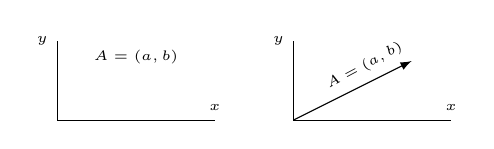
\begin{tikzpicture}
	\draw (0,1) -- (0,0) -- (2,0);
	\draw (3,1) -- (3,0) -- (5,0);
	\node[left] at (0,1) {\tiny$y$};
	\node[above] at (2,0) {\tiny$x$};
	\node[left] at (3,1) {\tiny$y$};
	\node[above] at (5,0) {\tiny$x$};
	\node at (1,0.8) {\tiny$A=(a,b)$};
	\draw[-latex] (3,0) -- (4.5,0.75);
	\node[rotate=28,above] at (4,0.5) {\tiny$A=(a,b)$};
\end{tikzpicture}
}
\end{figure} 

\begin{wrapfigure}{R}{0.2\textwidth}
	\centering
\scalebox{0.6}{%
\begin{tikzpicture}
	\draw[-Latex] (0,0) -- (2,1);
	\node[below] at (1,0.5) {$A$};
	\draw[-Latex] (0,0) -- (1,2);
	\node[left] at (0.5,1) {$B$};
	\draw[-Latex] (0,0) -- (3,3);
	\node[above,rotate=45] at (1.7,1.7) {$A+B$};
	\draw[dashed] (1,2) -- (3,3);
	\draw[dashed] (2,1) -- (3,3);
\end{tikzpicture}
}
\end{wrapfigure} 


If we use the second interpretation, then the first combination can be interpreted as \emph{vector addition}. The number $C$ is the vector obtained by the parallelogram law; i.e, it is the \emph{vector sum} of $A$ and $B$. 

The term ``first combination'' has now fulfilled its purpose. Henceforth we shall replace it by addition, meaning thereby precisely what has just been defined as the first combination, and write:
\[
C=A+B
.\] Similarly for subtraction. We define
\[
B-A \quad \text{ as } \quad B \ominus A;
\] i.e, the number which, added to $A$, gives $B$:
\[
	A+(B-A)=B
;\] or
\[
X=B-A
\]if
\[
A+X=B
.\] It is now easy to interpret the difference $B-A$ geometrically. 
\begin{wrapfigure}{R}{0.2\textwidth}
	\centering
\scalebox{0.9}{%
\begin{tikzpicture}
	\draw[-Latex] (0,0) -- (2,1);
	\node[below] at (0,0) {$O$};
	\node[below] at (1,0.5) {$A$};
	\draw[-Latex] (0,0) -- (1,2);
	\node[left] at (0.5,1) {$B$};
	\draw[-Latex] (2,1) -- (1,2);
	\node[right] at (1.5,1.5) {$B-A$};
\end{tikzpicture} 
}
\end{wrapfigure} 

Plot the vectors $A$ and $B$ with the same initial point $O$. Then $B-A$ is the vector whose initial point is the terminal point of $A$, and whose terminal point is the terminal point of $B$. 

The \emph{negative} of a number $A=(a,b)$ is defined as the number $(-a,-b)$, and is written $-A$:
\[
	A=(a,b), \quad -A=(-a,-b)
.\] 

We have here the two meanings of the minus sign discussed in the \emph{Real Variables}, p.42.

\emph{Multiplication}: The second combination is defined to correspond to the formal law of multiplication of imaginaries \ref{1.2mult}.

Let
\[
	A=(a,b), \quad B=(c,d)
\] be any two numbers of the system. By the \emph{second combination} is mean the mark:
\[
A\otimes B
.\] To it is attached the value
\[
C=A \otimes B
,\] where
\[
	C=(ac-bd,ad+bc)
.\] Thus
\[
	(a,b) \otimes (c,d) = (ac-bd,ad+bc)
.\] The second combination obviously obeys the Commutative Law:
\[
A\otimes B = B \otimes A
.\] It also obeys the Associative Law:
\[
	A\otimes (B \otimes C)=(A\otimes B)\otimes C
.\] The Distributive Law combines both the first combination and the second combination:
\[
	A\otimes (B+C)=(A\otimes B)+(A\otimes C)
.\] That it is true, is seen by direct calculation. The details are left to the student.

\emph{Division}: The second combination admits an inverse defined as follows. Let $A=(a,b)$ and $B=(c,d)$ be any two numbers of the system. It is required to determine a number $X=(x,y)$ such that
\[
A\otimes X=B
.\] This is always possible, and the result is unique, when
\[
A\neq A_0
.\] For, the equation is equivalent to the pair of equations:
\begin{align*}
	ax-by&=c\\
	bx+ay&=d
\end{align*} The determinant of these equations has the value:
\[
a^2+b^2
.\] Hence the truth of the statement.

When $A=A_0$, there is never a unique solution. If $B\neq A_0$, there is no number, $X$, which will satisfy the equation. If, on the other hand, $B=A_0$, the equation is satisfied by every number, $X$. 

\emph{Idemfactor}: The number
\[
	A_1=(1,0)
\] has the property that
\[
A_1\otimes A=A\otimes A_1=A
,\] no matter what number of the system $A$ may be. It is called the \emph{idemfactor} and is unique. It is the analogue of $A_0$ in the case of Addition. 

If $A\neq A_0$, and if $A'$ is determined by the equation:
\[
A\otimes A'=A_1
,\] then $A'$ is called the \emph{reciprocal} of $A$. It is the analogue of the negative of $A$ in the case of Addition.

The term ``second combination'' has now fulfilled its purpose. Henceforth we shall replace it by \emph{multiplication}, meaning thereby precisely what has just been defined as the second combination, and write:
\[
A\otimes B \quad \text{ as } \quad AB
.\] Division corresponds to the equation 
\[
AX=B, \quad A\neq A_0
.\] We write:
\[
X=\frac{B}{A}
.\] \emph{Relation of the Present Number System to the System of Real Numbers}: Any number $(a,b)$ of the present system can be written in the form:
\[
	(a,b)=(a,0)+(0,b)
.\] Thus the function of two variables has been broken up into the sum of two functions, each of a single variable. 

The sub-class consisting of the numbers $(a,0)$ constitute essentially a system of real numbers. For if we associate the number $(a,0)$ with the real number $a$:
\[
	(a,0) \sim a
,\]  not only will a one-to-one relation between the members of the above subclass and those of the system of real numbers be set up, but a holohedric isomorphism with reference to the four species will also result. For, from
\[
	(a,0) \sim a \quad \text{ and } \quad (b,0) \sim b
\] follows that
\begin{align*}
	(a,0)+(b,0) &\sim a+b\\
	(a,0) - (b,0) &\sim a-b
\end{align*} and furthermore:
\begin{align*}
	(a,0)(b,0) &\sim ab\\
	(b,0)(a,0) &\sim \frac{b}{a} \quad a\neq 0
\end{align*} It is, therefore, henceforth immaterial whether we write $(a,0)$ or $a$ in any expressions made up of numbers of the system. In particular, 
\[
	(0,b)=(b,0)(0,1)
\] and so we can write:
\[
	(0,b)=b(0,1)
.\] Hence the number $(a,b)$ of the system can be written in the form:
\[
	(a,b)=a+b(0,1)
.\] \emph{The Number}: $(0,1)=i$. The number $(0,1)$ has the property that
\[
	(0,1)(0,1)=(-1,0)=-1
.\] Denote this number by $i$. And now we see that we have a number system in which the algebraic equation:
\[
x^2+1=0
\] has a solution:
\[
x=i,\: -i
.\] Thus the number system which we have defined turns out to be identical with the \emph{System of Ordinary Complex Numbers}:
\[
a+bi, \quad i=\sqrt{-1} 
.\] It remains to mention explicitly a fundamental property of this arithmetic. A product $AB$ vanishes:
\[
AB=0
,\] when and only when one of the factors vanishes:
\[
A=0 \quad \text{ or } \quad B=0
.\] Of course, both may vanish.

We see how easily and naturally this system of numbers was evolved, to meet the formal requirement of the product:
\[
	(a+b\sqrt{-1} )(c+d\sqrt{-1} )=ac-bd+(ad+bc)\sqrt{-1} 
.\] It is a system of number-pairs-- pairs of real numbers, $a$ and $b$, just as the fractions were evolved from the natural numbers by forming number-pairs $(m,n)$; and again the negative numbers by forming pairs of negative numbers. There is nothing mystical or imaginary about the process. We see, too, how much simpler is the definition of $\sqrt{-1} $ than was the definition of $\sqrt{2} $. It was the definition of irrationals which was the most remote in all the extensions of the number system. 

The definition of ordinary complex numbers as pairs of real numbers is due to Sir William Rowan Hamilton, the inventor of quatrains, and dates from 1837.

\section{Formulas}

A complex number, $z=x+yi$, can be expressed in polar coordinates by the formula:
\[
	z=r\pbr*{\cos \phi +i\sin \phi } 
.\] The number $r$ is called the \emph{absolute value} of $z$ and is written as $\abs*{z} $:
\[
\abs*{z} =\sqrt{x^2+y^2} 
.\] The number $\phi $ has been called the ``amplitude'' and the ``argument'' of $z$. Neither term is satisfactory, nor has it been generally adopted. The term \emph{angle} would seem to be the simplest and most suggestive name for $\phi $, write:
\[
\phi =\text{arc} z
\] (read: ``angle of $z$''). For a given $z\neq 0$, there are an infinite number of determinations of $\phi $, differing from one another by multiples of $2\pi $. These are comprised, it is true, among the determinations of $\tan ^{-1}y /x$, but are not coextensive with them. Thus
\[
\text{arc } a=2n\pi , \quad n=0, \pm 1, \dots 
,\] where $z=a$ is a positive real number. But
\[
\tan ^{-1}0=n\pi , \quad n=0, \pm 1, \dots 
.\] The term \emph{pure imaginary} is applied to a number of the form $ci$, where $c$ is real. When
\[
z=x+yi
\] is represented by a point of the plane, the coordinate axes are called the \emph{axis of reals} and the \emph{axis of pure imaginaries}. The circle
\[
x^2+y^2=1, \quad \text{ or } \quad z=\cos \phi +i\sin \phi 
\] is known as the \emph{unit circle}. It is the locus of points for which $\abs*{z} =1$. 

The \emph{conjugate} of $x+yi$ is the number $x-yi$, and is frequently denoted by $\overline{z}$:
\[
z=x-yi
.\] The real part of $z$ is denoted by $\Re (z)$:
\[
	x=\Re (Z), \quad y=\Re \pbr*{\frac{z}{i}} 
.\] \emph{Geometrical Interpretation of Product and Quotient}: Let
\begin{align*}
	z_1&=r_1\pbr*{\cos \phi_1+i\sin \phi_1} \\
	z_2&=r_2\pbr*{\cos \phi_2+i\sin\phi_2} 
\end{align*} Then the product $z_1z_2$ is given by the formula:
\[
	z_1z_2=r_1r_2\sbr*{\cos \pbr*{\phi_1+\phi_2}+i\sin \pbr*{\phi_1+\phi_2}  } 
,\] as is shown by trigonometry.

\begin{wrapfigure}{r}{0.2\textwidth}
	\centering
\scalebox{0.9}{%
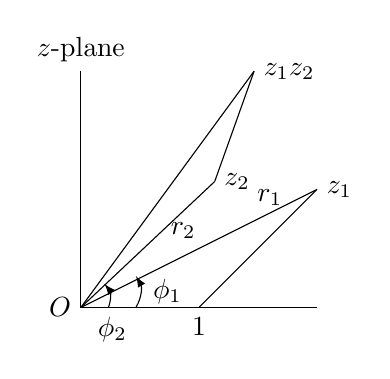
\begin{tikzpicture}
	\draw (0,3)--(0,0)--(3,0);
	\node[above] at (0,3) {$z$-plane};
	\node[below,left] at (0,0) {$O$};
	\draw (0,0)--(3,1.5);
	\node[right] at (3,1.5) {$z_1$};
	\draw (3,1.5)--(1.5,0);
	\node[below] at (1.5,0) {$1$};	
	\node at (2.4,1.4) {$r_1$};
	\draw (0,0)--(1.7,1.6) node[right] {$z_2$};
	\draw (1.7,1.6)--(2.2,3);
	\draw (0,0)--(2.2,3) node[right] {$z_1z_2$};
	\node[below] at (1.3,1.2) {$r_2$};
	\draw[bend right,-latex] (0.7,0) to (0.7,0.4);
	\node at (1.1,0.2) {$\phi_1$};
	\draw[bend right,-latex] (0.35,0) to (0.3,0.3);
	\node[below] at (0.4,0) {$\phi_2$};
\end{tikzpicture}
}
\end{wrapfigure}

The result admits a simple geometrical interpretation. Construct the triangle whose vertices lie at the points $0, 1, z_1$; and likewise the triangle whose vertices are at $0, z_2, z_1, z_2$. These triangle are similar. For the angles at $0$ are equal, and the including sides are proportional. 

Conversely, then: Given the numbers $z_1$ and $z_2$, construct the first triangle. Then draw a second triangle similar to the first, with vertex at $0$ and the side $\overline{0z_2}$ corresponding to the side $\overline{01}$. The third vertex will be at the point $z_1z_2$. 

\begin{wrapfigure}{R}{0.2\textwidth}
\scalebox{0.9}{%
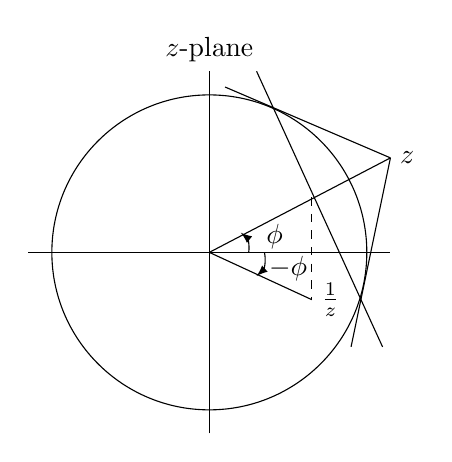
\begin{tikzpicture}
	\draw (0,2.3)--(0,0)--(2.3,0) node[above] at (0,2.3) {$z$-plane};
	\draw (0,-2.3)--(0,0)--(-2.3,0);
	\draw (0,0) circle (2);
	\draw (0,0)--(2.3,1.2) node[right] {$z$};
	\draw (2.3,1.2)--(0.2,2.1);
	\draw (2.3,1.2)--(1.8,-1.2);
	\draw (0.6,2.3)--(2.2,-1.2);
	\draw[bend right,-latex] (0.5,0) to (0.4,0.25);
	\node[right] at (0.6,0.2) {$\phi $};
	\draw (0,0)--(1.3,-0.6) node[right] {$\frac{1}{z}$};
	\draw[dashed] (1.3,0.7)--(1.3,-0.6);
	\draw[bend left,-latex] (0.7,0) to (0.6,-0.3);
	\node at (1,-0.2) {$-\phi $};
\end{tikzpicture}
}
\end{wrapfigure} 
Thus we have a geometrical construction for a product, just as we had a geometrical construction for a sum. In one respect, however, there is a difference. The geometric sum of two vectors was independent of the unit of length and the choice of axes; the geometric construction for the product of two vectors, however, is impossible until the unit of length and the axes have been determined. 

\emph{Reciprocals}: There is an elegant construction for the reciprocal of a complex number, $z$. Suppose the point representing $z$ lies outside the unit circle. Draw the tangents, and the chord determined by them. The distance of this chord from $O$ represents the absolute value of the reciprocal of $z$; and the angle of the reciprocal is the negative of the angle of $z$. The construction in the other cases can be left to the reader.

\emph{Tensors and Rotors}: The equation
\[
	z=r\pbr*{\cos \phi +i\sin \phi } =r e^{\phi i}
\] may be interpreted in an operational sense. To obtain the vector $z$ we may start with the vector $z=1$, the initial point being the origin, and then stretch it in the ratio of $r :1$. We thus obtain a vector of length $r$, lying along the positive axis of reals. Next, rotate this vector through the angle $\phi $. It now comes into coincidence with the vector $z$ we wished generate.

In the above equation, then, the first factor, $r$, may be thought of as a \emph{stretching factor}, or \emph{tensor}. The second factor, $e^{\phi i}$, \emph{rotates} the vector to which it is applied, and so is called a \emph{rotor}. 

The interpretation can be extended to any product,
\[
AB
.\] The effect of multiplying $B$ by $A$ is to \emph{stretch} the vector $B$ in the ratio of $\abs*{A} :1$, and then \emph{rotate} the vector thus obtained through the angle $\phi =\text{arc} A$ :
\[
AB=e^{\phi i}\abs*{A} B
,\] the order being:
\[
	\abs*{A} B; \quad \text{ then } \quad e^{\phi i}\pbr*{\abs*{A} B} 
.\] The order may be reversed:
\[
AB=\abs*{A} e^{\phi i}B
.\] \emph{Powers and Roots}: If
\[
	z=r\pbr*{\cos \phi +i\sin \phi } =r e^{\phi i}
,\] then
\begin{align*}
	z^2&=r^2\pbr*{\cos 2\phi +i\sin 2\phi } =r^2 e^{2\phi i}\\
	z^3&=r^3\pbr*{\cos 3\phi +i\sin 3\phi } =r^3e^{3\phi i}\\
	\vdots&\\
	z^n&= r^n \pbr*{\cos n\phi +i\sin n\phi } =r^ne^{n\phi i}
\end{align*}

It is now easy to solve the equation:
\[
z^n=A
.\] Let
\[
	A=\mathcal{A} e^{\alpha i}
,\] where $\mathcal{A} $ is real and $\mathcal{A} >0$. Then
\[
	z_k=\mathcal{A} ^{\frac{1}{n}} e^{\frac{\alpha +2k\pi }{n} i}, \quad k=0,1, \dots , n-1
.\] These points lie on a circle with radius $\mathcal{A}^{\frac{1}{n}}$, with its centre at the origin, and form the vertices of a regular inscribed polygon of $n$ sides, the angle of one root being $\alpha /n$. 

\emph{Roots of Unity}: In particular, the roots of unity are given by the equation:
\[
x^n=1
.\] They form the vertices of a regular polygon of $n$ sides inscribed in the unit circle, one vertex being at the point $z=1$.

\newdimen\R
\R=0.8cm
\begin{figure}[htbp]
\centering
\begin{tikzpicture}
    % Indicate the boundary of the regular polygons
	\draw circle (\R) ;
    	\draw (0:\R) \foreach \x in {120,240} {
            -- (\x:\R)
        } -- cycle (90:\R) node[above] {$n=3$};
\begin{scope}[xshift=2.5\R]
	\draw circle (\R);
	\draw (0:\R) \foreach \x in {90,180,...,359} {
            -- (\x:\R)
        } -- cycle (90:\R) node[above] {$n=4$} ;
	\end{scope}
	\begin{scope}[xshift=5.0\R]
	\draw circle (\R);
    \draw(0:\R) \foreach \x in {72,144,...,359} {
            -- (\x:\R)
        } -- cycle (90:\R) node[above] {$n=5$} ;
\end{scope}
    \begin{scope}[xshift=7.5\R]
	    \draw circle (\R);
        \draw (0:\R) \foreach \x in {60,120,...,359} {
                -- (\x:\R)
            }-- cycle (90:\R) node[above] {$n=6$} ;
    \end{scope}
\end{tikzpicture}
\end{figure}

\emph{Inequalities}: The inequality of greatest importance is the following:
\begin{equation}\label{triinq}
	\abs*{A+B} \underset{=}{<} \abs*{A} +\abs*{B} 
\end{equation} 


\begin{wrapfigure}{R}{0.2\textwidth}
\centering
\scalebox{0.8}{%
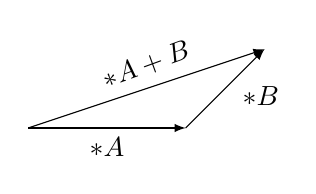
\begin{tikzpicture}
	\draw[-latex] (0,0)--(2,0);
	\draw[-latex] (2,0)--(3,1);
	\draw[-latex] (0,0)--(3,1);
	\node[below] at (1,0) {$\abs*{A} $};
	\node[right] at (2.6,0.4) {$\abs*{B} $};
	\node[rotate=20] at (1.5,0.8) {$\abs*{A+B} $};
\end{tikzpicture}
}
\end{wrapfigure}
Geometrically it is once obvious. It says that the length of one side of a triangle is less than the sum of the other two. But if the vectors $A$ and $B$ are collinear and have the same sense, then the lower sign holds. If they have the opposite sense, the upper sign holds.\footnote{For an arithmetic proof cf. \emph{Funktionentherie} I, p. 221.}

From \ref{triinq} it follows immediately that
\begin{equation}
	\abs*{A_1+\dots +A_n} \underset{=}{<}\abs*{A_1} +\dots +\abs*{A_n}.
\end{equation}
A further inequality is this:
\[
	\abs*{\cbr*{\abs*{A} -\abs*{B} } } \underset{=}{<}\abs*{A+B} 
.\] It can be deduced from \ref{triinq} by writing
\[
	\abs*{A+C} \underset{=}{<} \abs*{A} +\abs*{C} 
\] and then setting
\[
A+C=-B
.\] Thus
\[
	\abs*{B} -\abs*{A} \underset{=}{<} \abs*{A+B} 
.\] In this last inequality, interchange $A$ and $B$:
\[
	\abs*{A} -\abs*{B} \underset{=}{<} \abs*{A+B} 
.\] Hence the theorem.

\section{Exercises}
\begin{enumerate}
\item Show that the product of any number by its conjugate is equal to the square of its absolute value.
\item Let
	\[
		G(x)=a_0x^n+a_1x^{n-1}+\dots +a_n
	\] be a polynomial with real coefficients. Show that the conjugate of $G(z)$ is equal to $G(\overline{z})$. 
\item Let
	\[
		R(x)=\frac{f(x)}{\phi(x)} 
	\] be a rational function, the polynomials $f(x)$, $\phi (x)$ having real coefficients. Show that the conjugate of $R(z)$ is $R(\overline{z})$.
\item If the linear function
	\[
	\frac{az+b}{cz+d} ,\quad ad-bc\neq 0
	,\] takes on real values for three distinct real values of $z$, show that the coefficients can all be taken as real numbers. 

	Is it correct to say: ``The coefficients are all real''?
\item The function
	\[
	w=\log z
	\] is defined by the equation:
	\[
	z=e^{w}
	.\] Show that
	\[
	\log z=\log r+\phi i
,\] where 
\[
	z=r\pbr*{\cos \phi +i\sin \phi }
.\]
\item Show that
	\[
		\log (-1)=(2n+1)\pi i, \quad n=0, \pm 1, \dots 
	.\] 
\item Plot the points
	\[
		\log (-5-12i)
	.\] 
\item Show that
	\[
	\tan ^{-1}z=\frac{i}{2}\log \frac{i+z}{i-z} 
	.\] 
\item Show that
	\[
		\cos ^{-1}x=i\log \pbr*{x+\sqrt{x^2-1} } 
	,\] and obtain a similar formula for $\sin ^{-1}x$.
\item Compute:
	\[
	\sin ^{-1}2; \quad \cos \frac{i}{2}; \quad \tan ^{-1}2i
	.\] 
\item Solve the equation:
	\[
	x^n=-1
	.\] Plot the roots for the cases $n=2,3,4,5,6$.
\item Solve the equation
	\[
	x^3=-1
	\] by algebraic methods, and show that the results agree with those of Question 11.
\item Solve the equation:
	\[
	x^2+2ix-5=0
	,\] and plot the roots.
\item The same for
	\[
		x^2+(4-2i)x+(1-i)=0
	.\] 
\item Find all the roots of the equation:
	\[
	x^5=15
	,\] and plot them.
\item Prove the addition theorem:
	\[
	e^{u+v}=e^{u}e^{v}
	,\] for complex values of the arguments.

	Suggestion: write
	\[
	u=u_1+iu_2, \quad v=v_1+iv_2
	.\] 
\item Prove the addition theorem:
	\begin{align*}
		\sin (u+v)&=\sin u\cos v+\cos u\sin v\\
		\cos (u+v)&=\cos u\cos v-\sin u\sin v
	\end{align*} for complex values of the arguments.
\item State accurately under what conditions the equation
	\[
	\log u+\log v=\log uv
	\] is true for complex values of the arguments, and prove your statement.
\item If
	\[
	\abs*{A} <h \quad \text{ and } \quad \abs*{B} <h
	,\] show that
	\[
	\abs*{A+B} <2h
	,\] and, generally,
	\[
	\abs*{\pm A\pm B} <2h
	,\] where all four possible combinations of the $\pm$ sign are admitted.
\item Prove that
	\[
		\frac{1}{\sqrt{2} } \sbr*{\abs*{A} +\abs*{B} } \underset{=}{<} \abs*{a+bi} 
	,\] where $a$ and $b$ are real numbers.
\item If
	\[
	\abs*{A-B} <\epsilon \quad \text{ and } \quad \abs*{B-C} <\epsilon
	,\] show that
	 \[
	\abs*{A-C} <2\epsilon
	.\] 
\item If $\abs*{z} \underset{=}{<} h <1$, show that
	\[
		\abs*{\text{arc} (1+z)} \underset{=}{<} \sin ^{-1}h
	,\] where the numerically smallest value of $\text{arc} (1+z)$ is taken. 

	Suggestion: Draw a circle of radius $h$ about the point $1$. The point $1+z$ will lie in this circle.
\item A force can be represented by a vector. If forces $Z_1, \dots , Z_n$ act at a point and all lie in a plane, show that the resultant force, $Z$, is represented by the sum:
	\[
	Z=Z_1+\dots +Z_n
	.\] 
\item What is the condition that $n$ forces, lying in a plane and acting at a point, will be in equilibrium? 
\item The $n$ complex $n$-th roots of unity can be represented as vectors. Interpret the vectors as $n$ forces acting at a point. Hence show that the sum of the $n$ complex $n$-th roots of unity is equal to zero. 
\item Devise a somewhat similar proof to show that the sum of the $k$-th powers of the $n$ complex $n$-th roots of unity is $0$.
\item The theorem of partial fractions asserts that any proper fraction can be represented as the sum of the terms of the type:
	 \[
		 \frac{A_0}{(z-a)^n} +\frac{A_1}{(z-a)^{n-1}}+\dots +\frac{A_{n-1} }{z-a} , \quad A_0\neq 0
	.\] If the given fraction is the quotient of two polynomials with real coefficients, show that the fraction can be represented as the sum of expressions of the two types:
	\[
		\frac{A_0}{(x-a)^n}+\dots +\frac{A_{n-1} }{x-a} 
	\] and
	\[
		\frac{L_0x+M_0}{(x^2+px+q)^m} +\frac{L_1x+M_1}{(x^2+px+q)^{m-1}} +\dots +\frac{L_{m-1} x+M_{m-1} }{x^2+px+q} 
	,\] where all the coefficients are real and
	\[
	p^2-4q<0
	.\] Of the three quantities $A_0, L_0, M_0$, one or two may vanish, but not all three.
\end{enumerate}



\end{document}
